\section{Implementering}
I Simple Snake er der ikke brug for nogen menu, og det er derfor muligt at holde styringen af spillet meget simpel. Ved at definere de fire piletaster i \textit{Control}-klassen og en funktion der gør det muligt at bevæge sig på en bane som en torus, er alle styringskrav til Simple Snake opfyldt. Resten af spillet håndteres da i model-koden, mens view-koden gengiver spillet visuelt.
\newline

\subsection{Model}
Spillets model består af en række klasser, der tilsammen udgør spillets funktioner og objekter. Klassen \textit{Game} er selve spillets logik.

Klassen \textit{Field} bruges til at definere et punkt, som repræsenterer et felt på banen. Den fungerer på samme måde som \textit{Point}-klassen, hvor koordinatsystemet starter oppe i venstre hjørne. Forskellen mellem \textit{Point}- og \textit{Field}-klassen, er hvordan man kommer frem til et punkt. \textit{Point}-klassen går først ud ad x-aksen og derefter ned ad y-aksen, hvorimod \textit{Field}-klassen gør det i omvendt rækkefølge. Da hele spillepladen er delt op i rækker og kolonner, frem for en x- og y-koordinater, er \textit{Field} lettere at bruge for at undgå forvirring, da to-dimensionelle arrays også er opdelt i rækker og kolonner, hvor den første værdi repræsenterer rækker, mens den anden værdi repræsenterer kolonner. Vores \textit{Field} har også den fordel, at man ikke dynamisk kan ændre rækker og kolonner. Disse værdier er som datatypen String, låst fast, og nye koordinater kan kun opnås, ved at oprette et nyt \textit{Field}-objekt.
\newline

\textit{Field}-klassen har fået defineret en 'equals'-metode, der bruges til at undersøge om to objekter ligger på samme felt, f.eks. slangens hoved og maden. Maden er et \textit{Food}-objekt, som er defineret ved et \textit{Field}-objekt, idet den fylder præcist ét felt. Denne bliver oprettet i klassen \textit{Game}, hvor datafeltet 'position' afgør dens position.
\textit{Food} og \textit{Field} har kun to værdier i sig - en række og en søjle. Som tidligere nævnt, kan disse ikke ændres efter at de er blevet oprettet. Dette gør, at de kan returneres i getter-metoder, hvor det sikres, at udefrakommende klasser ikke ændrer dem. Nogle gange kan det være vanskeligt at resonere omkring kode, hvis alle objekter vilkårligt kan ændre hinanden. Immutable klasser sikrer, at objekter ikke har ændret sig. Dette gør, at det er umuligt for control-pakken at snyde spil-logikken.
\newline

Banen er oprettet i \textit{Game}-klassen, hvor der i konstruktøren også tjekkes om længden og højden af banen er af gyldige størrelse - dvs. værdier mellem 5 og 100. Her initialiseres spillerens score også, og der oprettes et Dimension-objekt, der skal repræsentere banen, et \textit{Snake}-objekt og et \textit{Food}-objekt. Hver klasse har de funktioner, der er relevante for dem, f.eks. \textit{getPosition} i \textit{Food}, der giver madens position i række/kolonne-koordinater. I \textit{Game}-klassen er også oprettet enum-værdierne for State: RUNNING, WON og LOST. Disse bruges af view-delen til at afgøre, hvad der skal vises i vinduet. 
\linebreak

Slangen selv er defineret ved klassen \textit{Snake}. Slangens krop består af en række felter, hvoraf det første er hovedet, og de resterende er kroppen med halen til sidst. Koordinaterne for disse Fields er gemt som elementer i en ArrayList kaldet 'positions'. Det første element er slangens første led, hovedet, det andet element er slangens andet led osv.
\newline

Slangens flyttes ved at kalde dens 'move'-metode. Metoden signalerer internt til \textit{Game}-objektet, at slangen har bevæget sig. Det gøres med metoden 'snakeHasMoved'. 'Move' er et enum, som betegner slangens handling: om slangen ikke kan bevæge sig, spiser maden, er død eller bevæger sig, henholdsvis EAT\_NECK, EAT\_FOOD, EAT\_BODY og NORMAL. Først tjekkes, at slangen ikke bevæger sig ind i sin hals. Hvis det sker, signaleres EAT\_NECK, og der returneres og ventes igen på nyt kontrol-input. Det undersøges derefter, om der er mad på samme felt som slangehovedets nye placering. Før slangen faktisk bevæger sig, beregnes altså det felt som spilleren flytter hovedet ind i, \textit{når} slangen rykker sig. Dette gøres når 'move'-metoden kalder på 'findMovePosition'-metoden, der tager en Direction som input, og beregner den nye position ud fra hovedets nuværende position. Hvis den nye position ligger inde for banen, returnerer metoden blot et felt med de koordinater. Ligger et koordinat uden for banens grænser, returneres i stedet koordinatet på den modsatte side af banen.
Dette beregnede felt kan nu sammenlignes med \textit{Food}-objektets koordinater, og er disse ens, signaleres EAT\_FOOD, et nyt hoved tilføjes i 'snake'-ArrayListens index 0 med hovedets nye koordinater, maden forsvinder, og der returneres, hvorefter der igen ventes på nyt konrol-input. Hvis ikke maden har samme koordinater som hovedets nye felt, undersøges der, om den nye placering indeholder slangens krop. Dette gøres ved at undersøge om snake-ArrayListen - pånær det sidste element - indeholder et element der har de samme koordinater som hovedet. Hvis en af listens elementer har samme koordinater som hovedet, signaleres EAT\_BODY. Hvis ikke, tilføjes et nyt hoved på det nye felt og det sidste element i ArrayListen fjernes. Dette giver en illusion af at slangen har rykket sig et felt frem.
\newline

Signalerne fra 'Move'-enum, kan nu bruges til at bestemme spillets tilstand. Dette gøres i \textit{Game}-klassens 'snakeHasMoved'-metode, der sætter State til WON eller LOST, eller opretter nyt mad, hvis det gamle er spist. 'findFoodPosition'-metoden i \textit{Game}-klassen sikrer, at maden altid placeres på et gyldigt felt, dvs. et felt der ikke er udfyldt af slangen. For at sikre dette, placeres maden først på et tilfældigt felt inden for banens rammer, hvorefter der undersøges om et af slangens led i 'snake'-ArrayListen har samme koordinater som madens felt. Er dette tilfældet, gives maden et nyt felt, indtil det lander på et felt uden slangens krop. Er slangen tilpas stor, er dette dog ikke effektivt, da der er stor sandsynlighed for at ramme et felt, der er optaget af slangen. Af denne årsag undersøger metoden først, om slangen fylder mere end halvdelen af banen. Er dette tilfældet, laves der i stedet en liste med alle tomme felter vha. en indlejret for-løkke, der løber gennem alle banens rækker og kolonner, hvorefter et tilfældigt element i listen vælges som madens position.

\subsection{View}
Brugergrænsefladen er samlet i view-klassen \textit{View} der nedarver fra JFrame. I \textit{View}s konstruktør oprettes et \textit{ScorePanel}-objekt, der placeres øverst i vinduet, og et \textit{BoardPanel}-objekt, der placeres under det i et BorderLayout. Board-panelet viser selve banen med slangen og maden, der begge er vist ved farvede firkanter, mens score-panelet, viser scoren.
\newline

\textit{ScorePanel}-klassen nedarver fra JPanel og implementerer Observer. Klassen har en 'update'-metode, som signalerer at panelet skal optegnes påny, hver gang noget ændrer sig \textit{Game}, da denne klasse har fået tilføjet score-panelet som Observer. 'paintComponent'-metoden benyttes til at tegne score-tekstfeltet. \textit{BoardPanel} nedarver også fra \textit{JPanel} og implementerer Observer, for at den også kan registrere ændringer i \textit{Game}-klasse. Den består af en række 'draw'-metoder, samt en 'paintComponent'-metode, der kalder på 'draw'-metoderne for at tegne alle spillets komponenter på spillets bane og spillets bane selv. Disse tegnes med Graphics2D, der tegner en rektangel pr. felt.
\newline

Da spillepladen skal være mellem $5\times 5$ og $100\times 100$ felter, kan det skabe problemer, hvis spilleren ikke kan justere størrelsen på vinduet eller banen. Vinduet kan være for stort til at passe på en gennemsnitlig computerskærm eller for lille til at gøre hele banen synlig. Det er derfor nødvendigt at gøre spillets vinduesstørrelse og selve bane- slange- og æble-størrelsen fleksibel. Derfor beregnes en passende feltstørrelse med metoden 'getWindowRectangle' i \textit{BoardPanel}, der beregner den størst mulige længde på hvert led - afhængig af vinduets størrelse og antal felter på hvert led af banen. Når feltets bredde og højde er udregnet, kan denne rektangel nu bruges til at tegne banen, slangen og æblet.
På \figref{udstrakt} kan man se, at længden og højden af et felt tilpasser sig vinduesstørrelsen og udvider sig på det led, som vinduet strækkes på. Det kan derfor risikeres, at felterne og banen bliver aflange og ikke særlig pæne at spille på.

\begin{figure}[h]
	\centering
	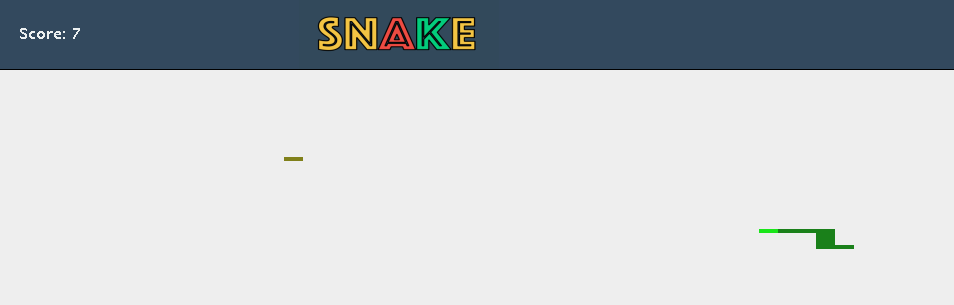
\includegraphics[width=0.8\textwidth]{WindowSize.png}
	\caption{\figlab{udstrakt}\textit{Simple Snake med udstrakte felter}}
\end{figure}

\subsection{Control}
I Simple Snake er der ikke brug for nogen menu, og det er derfor muligt at holde styringen af spillet meget simpel. \textit{Control}-klassen nedarver fra KeyAdapter og implementerer derfor metoden 'keyPressed', som kaldes hver gang, der tastes på tastaturet. Hvis tasten er en af de fire piletaster, kaldes metoden 'move' i \textit{Snake}-klassen. For at \textit{Control}-klassen registrerer tastatur-input, tilføjes den som keyListener til \textit{View}-klassen.